\documentclass[12pt]{article}

\usepackage[english]{babel}
\usepackage[utf8x]{inputenc}
\usepackage{amsmath}
\usepackage{graphicx}
\usepackage{authblk}
\usepackage{natbib}
\usepackage{hyperref}
\bibpunct{(}{)}{;}{author-year}{}{,}

\title{Host diversity increases symbiont diversity and reduces transmission}

\author[1]{Maxwell B. Joseph} 
\author[2]{Joseph R. Mihaljevic}
\author[1]{Pieter T. J. Johnson}
\affil[1]{Ecology and Evolutionary Biology, University of Colorado, Boulder}
\affil[2]{Ecology and Evolution, University of Chicago}
\date{}
\renewcommand\Affilfont{\itshape\small}

\begin{document}
\maketitle

\begin{abstract}
Your abstract.
\end{abstract}

\section*{Introduction}

Debate around effect of host diversity on disease. 
Increased availability of microbial data. 
Need for theoretical framework to make sense of data and predict future observations.

General strategy: 
- formalize the notion that host infection dynamics potentially have similarities to free living metacommunity dynamics
- develop a model that can capture the complexity of multi-host, multi-symbiont systems
- advantages (better realism, adequate complexty)
- disadvantages (less tractable than a simple analytical mathematical model)

\section*{Methods}

We developed a stochastic continuous-time agent-based model for the dynamics of host-symbiont communities in local habitat patches that are made up of a finite number of cells that may be occupied by hosts. 
The local habitat patches are all considered to be equivalent with respect to host colonization, reproduction, and death. 
Multiple host species exist within a regional pool, and each patch experiences a constant rate of host colonization, which is equal for all host species, and there is no displacement of occupying hosts by colonizing hosts. 
Hosts vary in traits that are relevant to symbiont infection, but the communities are otherwise neutral, in that all host species have equal colonization, reproduction, and death rates. 
Once a host colonizes a patch, it then has some rate of reproduction and of death that is constant among host species.
Offspring attempt to disperse to a random habitat patch, and if it is unnoccupied, they successfully colonize.

Multiple types of symbionts occur in the regional pool and attempt to colonize host individuals with a constant rate. 
Host species vary in traits relevant to symbiont establishment probability. 
We assume for simplicity that this variation is unidimensional, as would be the case if there were one primary niche axis for the symbionts, e.g. pH of the host gut. 
Symbiont niches are represented as univariate Gaussian functions with niche optima and breadths (means and variances, respectively), such that the probability of successful establishment $p_e$ on an individual host is a function of the host's value along the niche axis (Figure \ref{fig:niche}). 
Symbionts have the potential to establish when a susceptible host contacts an infected host, or when a symbiont from the regional pool attempts to colonize a susceptible host in a local community.
Each symbiont in the regional pool has the same probability of colonizing across the range of possible host conditions as a result of adjusting the niche functions of symbiont species with niche optima near the boundaries of  the niche space of the regional pool \citep{Allouche2012}.
 
Every individual host has some constant probability of a symbiont from the regional pool attempting to infect, with an infection establishment probability $p_e$ from the symbiont niche function. 
If a symbiont successfully colonizes a host, it becomes part of the local community and can either be extirpated through host recovery or persist by transmitting to other hosts (Figure 2). 
Every infected host has a recovery rate that is assumed constant across all species. 
Hosts contact each other with rate $\phi$, also assumed constant across host species, so that the overall rate of contacts between susceptible and infected individuals is $\phi S I$, where $S$ is the number of susceptible hosts, and $I$ is the number of infected hosts.
Conditional on a contact, the infected host passes the symbiont infection to the susceptible host probability $p_e$, derived from the symbiont niche function.
In this way, host species that are functionally similar are more likely to exchange symbionts.

We implemented this model via stochastic simulation, generating continuous-time Markov chains in high-dimensional space, where the dimensions represent the states: number of hosts of each species, and the symbionts that infect each individual. 
Although continuous-time Markov processes are more difficult computationally than discrete-time formulations, they have the advantage of not requiring an arbitrarily specified order of events at each time step. 
The order of events emerges from the rates of each potential process via the Gillespie algorithm \citep{Gillespie1976}. 
Given the state of the system at any time point, every potential event that could happen is represented by some rate $r_e$ for events $e = 1, ..., E$. 
The total rate of events is simply the sum of the component rates $r_{tot} = \sum_{1}^{E} e_r$, and the time until an even happens is exponentially distributed, with overall rate parameter $r_{tot}$. 
This provides a way to generate the timepoints stochastically, and given some time of an event happening, the specific event is be selected with probability $e_r / r_{tot}$. 

We were interested broadly in the effect of host functional diversity on symbiont transmission and richness within a local host community. 
In addition, we explored the effect of symbiont niche breadth ($\sigma$ in Figure \ref{fig:niche}), and the effect of infection on host fitness, described below. 
These questions lead to six different simulation experiments. 
The first explores the effect of host functional diversity on transmission and symbiont richness when all symbionts are functionally equivalent and commensal.
The second allows symbiont niche width to vary among simulated realizations, but assumes that the niche width of all symbionts is equal within a simulation run. 
The third varies the effect of symbiont infection on host survival, varying across simulation runs but equal among symbionts within a run. 
The fourth varies symbiont niche width within and across simulation runs so that the regional pool of symbionts includes a combination of specialists and generalists.
The fifth varies symbiont fitness effects within and across runs so that the regional pool includes parasites and mutualists.
The sixth and final experiment allows both niche width and fitness effects to vary within and across runs so that the regional pool of symbionts includes a range of specialist and generalist parasites and mutualists. 
Details of how the specific parameters were chosen for each of these experiments is provided in the supplemental material, and we also provide all code to replicate the analysis at \url{https://github.com/mbjoseph/abm}.

\section*{Results}

In our first experiment all symbionts were commensal and had equal niche widths. 
Across 1000 simulated local host communities, host functional diversity decreased symbiont transmission while increasing symbiont richness (Figure \ref{f2}). 
Symbiont diversity increased non-linearly with host functional diversity, with the fastest increases occurring at low levels of host functional diversity. 
While symbiont transmission was lower on average in communities with high symbiont diversity, there was one instance in a low-diversity host community in which no symbionts could colonize, because the range of host resources that were available in the local community was outside the optimal niche space of the symbionts in the regional pool. 
In other words, symbionts attempting to colonize had very low probabilities of establishment in the hosts, such that across the range of timesteps, no symbionts succeeded in colonizing the local community. 

In our second experiment where the niche width of symbionts varied among simulations but was constant among species within each simulation, host diversity still increased symbiont richness and decreased transmission, but these relationships were strongly moderated by symbiont niche width (Figure \ref{f3}). 
The increases in symbiont richness with host richness were still non-linear, but they shifted from being concave down to concave up as symbionts became more generalized. 
Transmission consistently decreased as host communities became more functionally diverse, but as symbiont niche width increased, there were fewer outlier communities with extremely low transmission, because it becomes less likely that any particular host community will have a range of resources available that cannot be exploited by symbionts in the regional pool because of a mismatch with their niche space.

In our third experiment where the fitness consequences of infection varied among simulations, host diversity still increased symbiont richness and reduced transmission, but parasites had lower richness and transmission on average compared to mutualist and commensal symbionts (Figure \ref{f4}). 
This is likely because parasites restrict their own transmission by killing hosts, making it more difficult to persist in a local host community. 
As a result, richer host communities still can be colonized by more parasitic symbiont species, but these communities will have more depauperate symbiont communities relative to communities comprised of less virulent symbionts. 

When symbiont niche width varied within communities, host diversity still increased symbiont richness, but the effects of host diversity on symbiont transmission were more subtle (Figure \ref{f5}). 
Specialist symbionts had the highest transmission rates in low-diversity communities, but had relatively low transmission in more diverse host communities. 
Generalist symbionts actually had higher transmission in the high diversity host communities, and lower transmission in less diverse host communities, consistent with the idea that specialist symbionts can outcompete generalists. 
In addition, mean niche breadth in the symbiont community increased with host functional diversity, such that diverse host communities contained more generalist symbionts than low diversity host communities. 

When symbionts varied in fitness effects, host diversity increased symbiont richness, and reduced transmission, but the reduction in transmission was more pronounced for parasitic than mutualistic symbionts (Figure \ref{f6}). 
Interestingly, extremely mutualistic symbionts had a lower peak transmission in low diversity communities than moderately mutualistic symbionts, because host were so long-lived that the majority habitat patches in the lowest diversity communities were occupied by extremely long-lived, infected hosts, such that there were fewer susceptible hosts available for transmission. 
There were no clear patterns with the mean fitness effect as a response to host functional diversity. 

When symbionts varied in fitness effects and niche breadth, host diversity still increased symbiont diversity and reduced transmission (Figure \ref{f7}). 
Mutualistic symbionts nearly always had higher transmission than parasitic symbionts, and on average, symbionts in the local communities were mutualistic. 
Furthermore, low diversity host communities had more specialist symbionts than high diversity communities, which primarily consisted of generalists. 
Both of these findings are consistent with the component cases when fitness effects and niche breadth are the only varying parameters.

\section*{Discussion}

Across a wide range of situations, host functional diversity consistently increased symbiont diversity and reduced transmission in our model. 
Fitness consequences of infection and symbiont niche breadth regulated the degree and to a lesser extent the shape of these relationships.
In general, we expect that across replicated communities in nature, that all else being equal, host communities that are low in functional diversity will have relatively low symbiont richness but high transmission, and that specialist symbionts may be more likely to occur in high abundance. 
In contrast, host communities that are incredibly diverse are more likely to have diverse symbiont communities with lower mean transmission rates, and also more generalist symbionts. 

Connections to existing theory
\begin{itemize}
	\item Dobson and our paper
	\item Allouche
\end{itemize}

Connections to empirical results
\begin{itemize}
	\item See Dunn et al. 2010 for non-linear relationship
	\item See Rotstock et al. 2014 for similar resolution of paradox
\end{itemize}

Shortcomings of this approach
\begin{itemize}
	\item Many parameters
    \item Constraints on model realism
    \item Hard to validate
\end{itemize}

Future directions
\begin{itemize}
	\item Experimental validation on simple hosts
    \item Evaluation at multiple scales (metacommunity)
\end{itemize}

Dynamic host communities
- difference between potential vs. realized host richness
- not as strong unimodal relationships observed, because it's very unlikely to have tons of very small, very different host populations (small populations face a higher risk of stochastic extinctions)



\bibliographystyle{plainnat}
\bibliography{Mendeley}

\newpage

\begin{figure}[ht]\centering
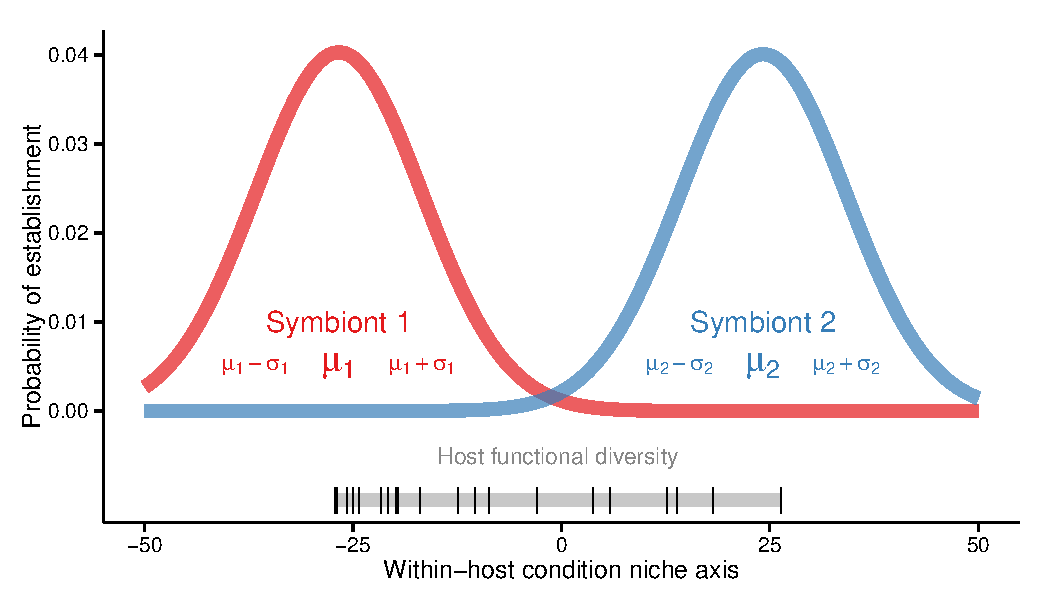
\includegraphics[width=\linewidth]{fig/niche.pdf}
\caption{Conceptual diagram illustrating the niche space of symbionts along a univariate host-condition axis (the x-axis). Each host species in a local host community is assigned one particular value, shown as vertical bars. The range of the values represents the host functional diversity represented in the local community. Here two symbiont species have equal niche breadths $\sigma$ but different optima $\mu$, which together define the Gaussian function that relates host condition to the probability of symbiont establishment, conditional on an infection attempt.}
\label{fig:niche}
\end{figure}

\newpage

\begin{figure}[ht]\centering
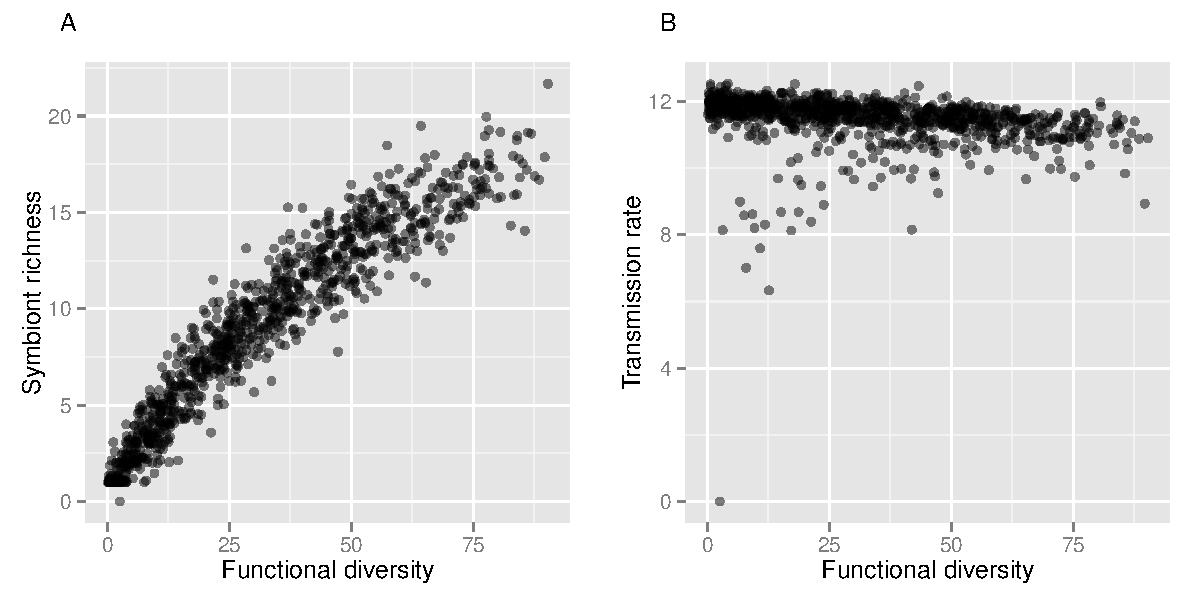
\includegraphics[width=\linewidth]{fig/fig1.pdf}
\caption{Commensal symbionts, all same niche width}
\label{f2}
\end{figure}

\newpage

\begin{figure}[ht]\centering
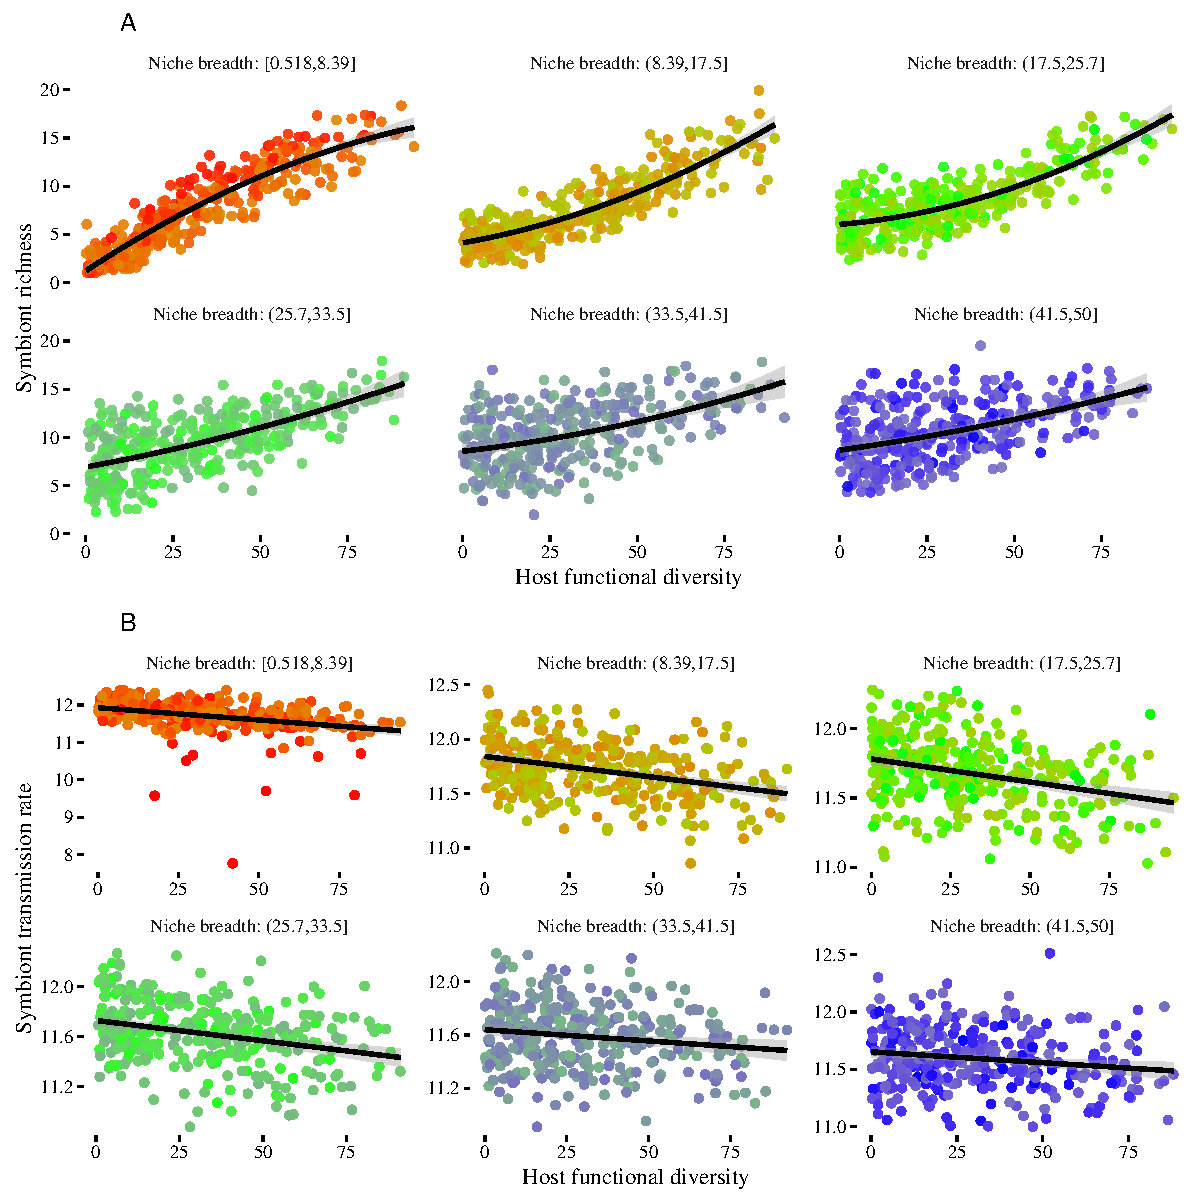
\includegraphics[width=\linewidth]{fig/fig2.pdf}
\caption{Varying niche width, but constant within symbiont community}
\label{f3}
\end{figure}

\newpage

\begin{figure}[ht]\centering
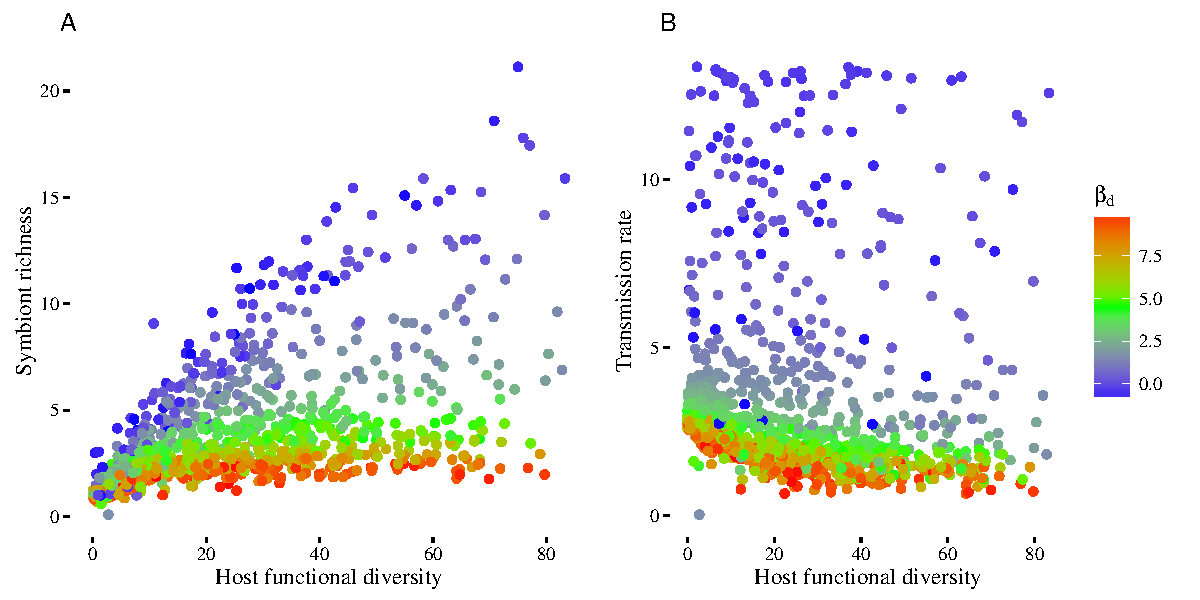
\includegraphics[width=\linewidth]{fig/fig3.pdf}
\caption{Varying fitness consequences, but constant within symbiont community}
\label{f4}
\end{figure}

\newpage

\begin{figure}
\centering
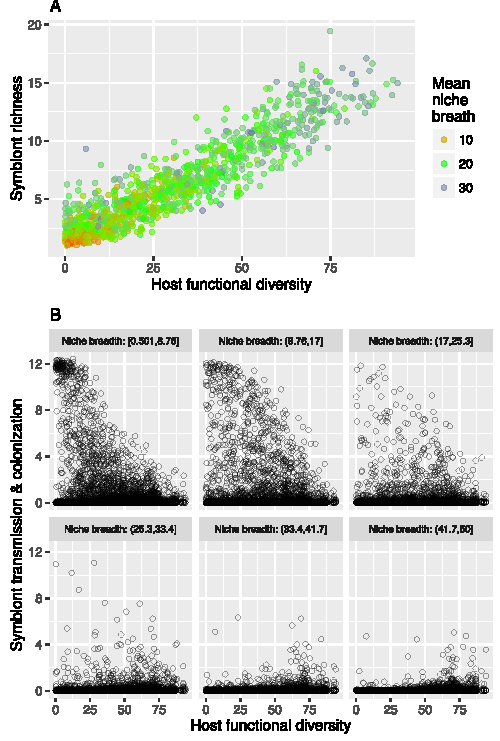
\includegraphics[width=\textwidth,height=\dimexpr\textheight-4\baselineskip-\abovecaptionskip-\belowcaptionskip\relax,
keepaspectratio]{fig/fig4.pdf}
\caption{Mixed niche breadths within symbiont community}
\label{f5}
\end{figure}

\newpage

\begin{figure}[ht]\centering,
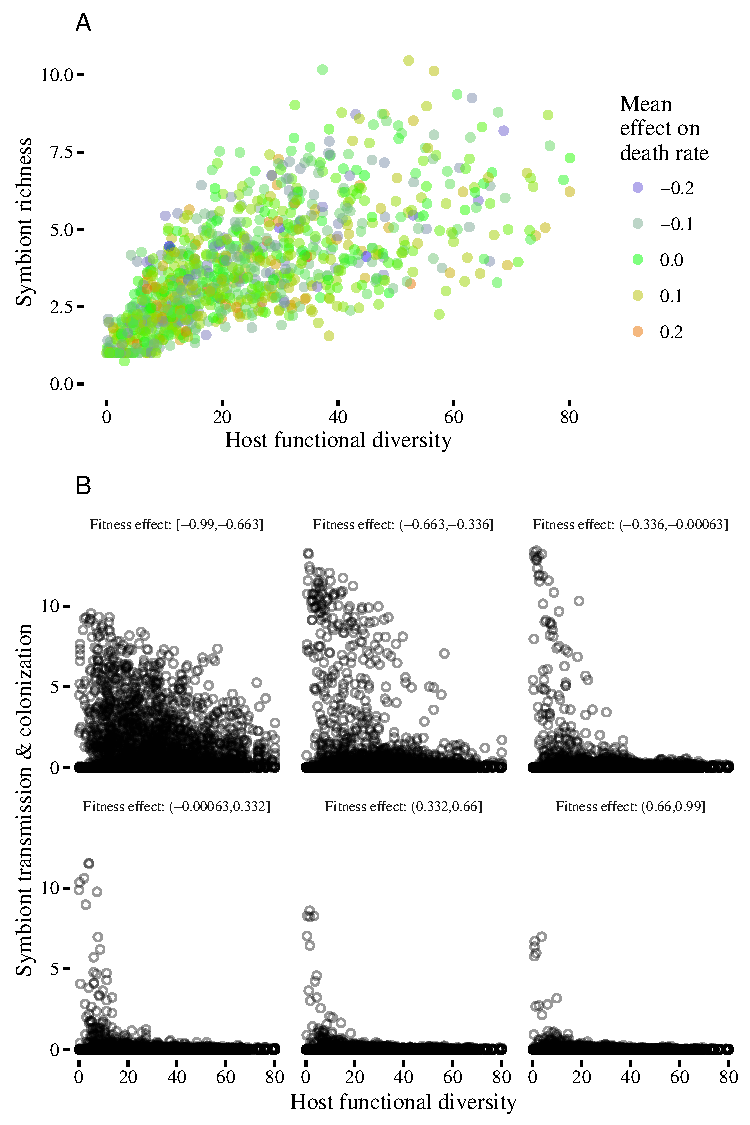
\includegraphics[width=\textwidth,height=\dimexpr\textheight-4\baselineskip-\abovecaptionskip-\belowcaptionskip\relax,
keepaspectratio]{fig/fig5.pdf}
\caption{Mixed fitness consequences within symbiont community}
\label{f6}
\end{figure}

\newpage

\begin{figure}[ht]\centering,
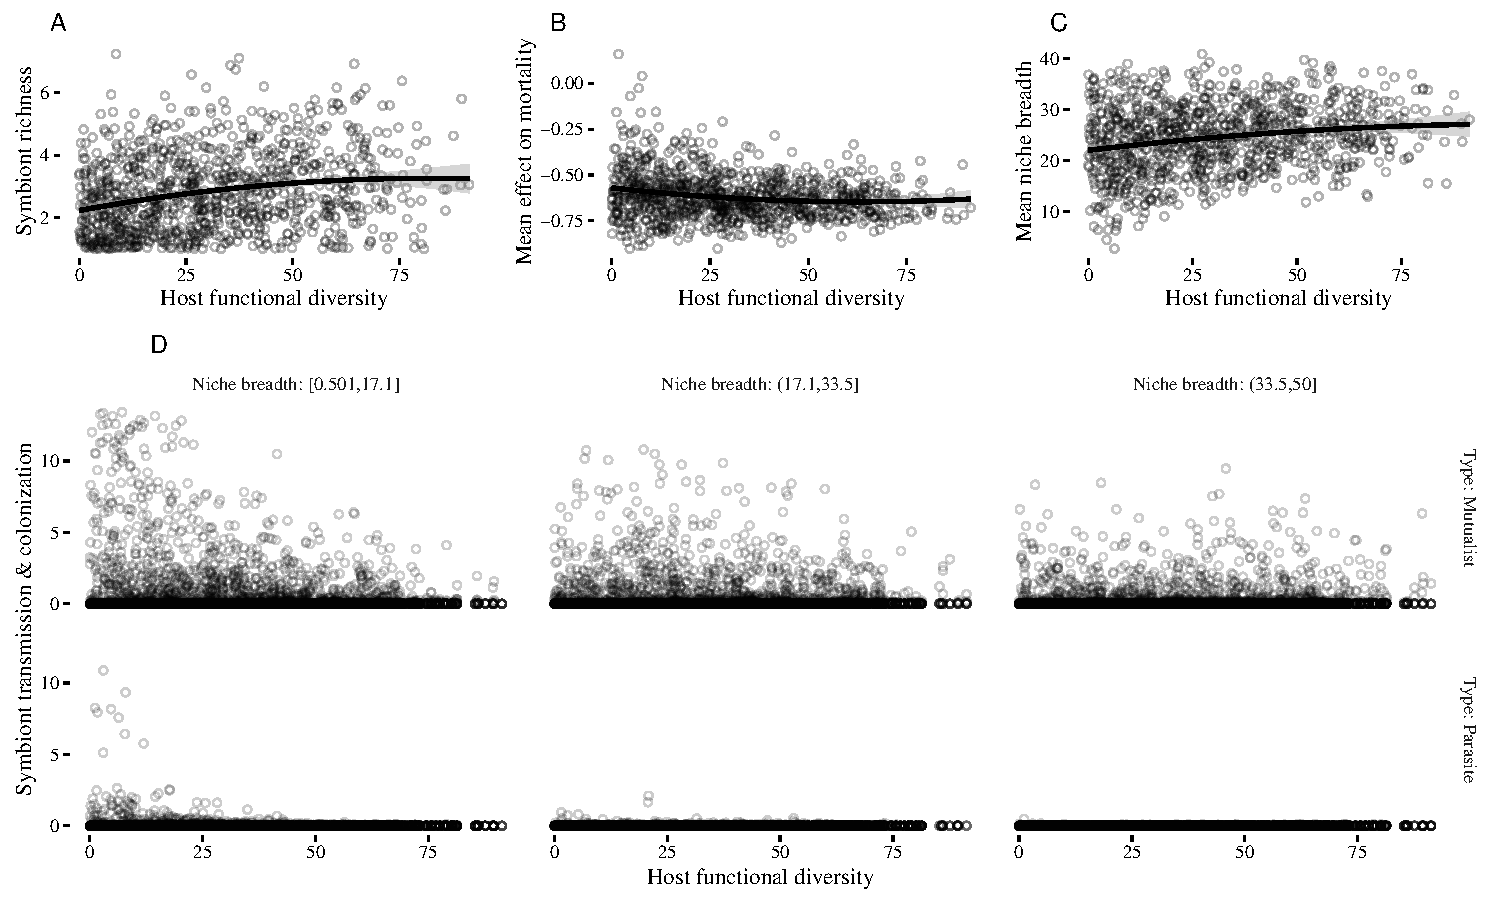
\includegraphics[width=\textwidth,height=\dimexpr\textheight-4\baselineskip-\abovecaptionskip-\belowcaptionskip\relax,
keepaspectratio]{fig/fig6.pdf}
\caption{Mixed niche breadths and fitness consequences}
\label{f7}
\end{figure}

\newpage

\end{document}